\chapter{スクリプト拡張機能}\label{ch:se}

\section{目的}
変換ルール、可視化ルールの機能は限定的であるため、複数のイベントに基づ
く可視化を行なえなかった。例えば、ある時間に起動しているタスクの数を数
える必要のあるCPU使用率の可視化を行なえない。

しかし、先行リリースなどによって収集した要求のなかで、こういった複数の
イベントに基づく可視化を行ないたいという要望が強かった。そのため、
複数のイベントに基づく可視化の実現するための機能追加を行なう。

\section{設計}
\subsection{変換・可視化の実現}
複数のイベントに基づく可視化の実現する方法について、
次の3つの方針を検討、比較した。

1つ目は、変換ルールと可視化ルールを拡張し、複数のトレースログに基づく可
視化を記述できるようにする方針である。既存のルールを拡張するので、すで
にルールの記述法を習得している利用者の学習コストが低い。しかし、可視化
ルールが複雑化しているため、可読性と後方互換性を保ちつつ、拡張を加える
のは困難である。またルールの処理に関するソースコードが複雑化しているた
め、変更を加えるのが難しい。

2つ目は、標準トレースログ間の変換を記述するための言語を実装し、変換処理
と可視化処理の間に標準形式トレースログを変形する処理を追加する方針であ
る。ルールの複雑化や互換性の維持のためのコストを避けることができ
る。また、既存の処理と独立して実装できるため、ソースコードの複雑さを避けられる。
しかし、利用者は新たな言語の学習が必要となる。また、新たな言語を設計
する必要があるため、実装コストも高い。

3つ目は、外部のプロセスによって標準形式トレースログへの変換と図形データ
の生成を行なえるようにTLVを拡張する方針である。変換処理は外部プロセスで
行なうため、任意のプログラミング言語で記述できる。利用者が自分の使える
プログラミング言語で変換を記述できるため、学習コストもそれほど高くない。
また、既存のプログラミング言語を利用できるため、言語設計のコストを避け
られる。既存の処理と独立して実装できるため、ソースコードの複雑さを避け
られる。

上記の点を考慮し、
利用者の学習コストと実装コストを低くするために、
3つめの外部プロセスによる変換の実現を選択した。

% ------------------------------
\subsection{変換ルール・可視化ルールの拡張}
変換・可視化処理を行なう外部プロセスを指定する方法について、次の2つの方
針を検討、比較した。

1つ目は、外部プロセスを指定するためのルールファイルを追加する方針である。
既存の変換ルール・可視化ルールとの互換性などを考慮する必要がないが、利
用者は新たに学習する必要がある。また、新たなルールファイルを追加するた
め実装・保守コストが高い。さらに、旧ルールファイルと新ルールファイルが
衝突した際の処理も必要となる。

2つ目は、既存の変換ルール・可視化ルールの拡張し、変換を行なう外部プロセ
スを指定できるようにする方針である。すでにルールの記述法を習得している
利用者の学習コストが低いが、既存のルールとの互換性などを考慮する必要が
ある。ただし、既存のルールはそれほど複雑ではないため、互換性を保つため
のコストはそれほど高くない。また、既存の処理を拡張することで実装できる
ため、実装コストが低い。

上記の点を考慮し、
2つめの既存のルールの拡張を選択した。

\section{実装}
\subsection{TLVファイルの拡張}
フェーズ3直後のTLVは、\figref{fig:se-before}のように、中間形式であるTLVファイルは、
図形データを保持していない。TLVファイルを開く際に、
TLVファイル内の標準形式トレースログに可視化ルールを適用し、
図形データを生成した後、描画を行なっていた。

このTLVファイルのまま、図形データの生成を外部プロセスで行なうようにする
と、TLVファイルを開く際に外部プロセスを実行する必要がある。しかし、外
部プロセスを実行する環境は、全ての計算機上には用意されていないため、
TLVファイルの可搬性が失なわれる。また図形データ生成の結果は常に同一であるに
もかかわらず、毎回ファイルを開く際に図形データ生成が行なわれるため効率が悪
い。

そこで、TLVを\figref{fig:se-after}のように変更し、TLVファイルに図形データ
も保持し、ファイルを開く際はその図形データを描画するようにする。

\begin{figure}
\centering
\includegraphics[width=\textwidth]{se-before.eps}
\caption{変換機能拡張前のTLVの変換処理}\label{fig:se-before}
\end{figure}

\begin{figure}
\centering
\includegraphics[width=\textwidth]{se-after.eps}
\caption{変換機能拡張後のTLVの変換処理}\label{fig:se-after}
\end{figure}

\subsection{変換ルールの拡張}
変換ルールファイルを変換に用いる外部スクリプトを指定できるように拡張する。

変換に用いる外部スクリプトを指定するために、変換ルールファイルには表
\ref{conv}の要素を用いる。\figref{outside}のように、\verb!arguments!を
用いて外部スクリプトを指定する。あるいは、\figref{inline}のように
\verb!script!を用いて変換ルールファイル内にスクリプトを直接記述すること
可能である。

\begin{figure}
\begin{lstlisting}
{
  "asp2": {
    "$STYLE": "script",
    "fileName": "c:/cygwin/bin/ruby",
    "arguments": "conv.rb",
  }
}
\end{lstlisting} % $
\caption{外部スクリプトを指定する変換ルールの例}\label{outside}
\end{figure}

\begin{figure}
\begin{lstlisting}
{
  "asp2": {
    "$STYLE": "script",
    "fileName": "c:/cygwin/bin/ruby",
    "arguments": "{0}",
    "script" : "puts '[1]TASK1.state=RUNNING'"
  }
}
\end{lstlisting} % $
\caption{直接記述する変換ルールの例}
\label{inline}
\end{figure}

\begin{table}[hb]
\centering
\caption{変換ルールに追加された要素}\label{conv}
\begin{tabular}{|c|l|}
\hline
要素 & 内容  \\\hline
\verb!$!STYLE & 旧ルールと区別するための要素。常にscriptと記述する  \\
fileName  & スクリプトを実行する処理系 \\
arguments & 実行時に渡される引数。\verb!{0}!は一時ファイル名に置き換えられる。 \\
script    & 変換スクリプトの内容 \\
\hline
\end{tabular}
\end{table}

\subsection{可視化ルールの拡張}
\begin{figure}
\begin{lstlisting}
[
 {
   "Type":"Rectangle",
   "Size":"100%,80%",
   "Pen":{"Color":"ff00ff00","Width":1},
   "Fill":"6600ff00"
 },
 {
   "Type":"Rectangle",
   "Size":"100%,80%",
   "Pen":{"Color":"ff00ff00","Width":1},
   "Fill":"6600ff00"
 }
]
\end{lstlisting}
\label{array}
\caption{図形データの例}
\end{figure}

可視化に用いる外部スクリプトを指定するために、可視化ルールファイルに
\figref{viz}の要素を用いる。\figref{outside-viz}のように、
\verb!arguments!を用いて外部スクリプトを指定する。あるいは、
\figref{inline-viz}のように\verb!script!を用いて可視化ルールファイル内
にスクリプトを直接記述することも可能である。

\begin{figure}
\begin{lstlisting}
{
  "asp2":{
     "VisualizeRules":{
        "taskStateChange":{
           "Style": "script",
	   "DisplayName":"状態遷移",
   	   "Target":"Task",
           "FileName": "c:/cygwin/bin/ruby",
           "Arguments": "viz.rb",
        }
    }
  }
}
\end{lstlisting}
\caption{外部ファイルを指定する可視化ルールの例}\label{outside-viz}
\end{figure}


\begin{figure}
\begin{lstlisting}
{
  "asp2":{
     "VisualizeRules":{
        "taskStateChange":{
           "Style": "script",
	   "DisplayName":"状態遷移",
   	   "Target":"Task",
           "FileName": "c:/cygwin/bin/ruby",
           "Arguments": "{0}",
           "Script" : "puts '{ \"Type\":\"Rectangle\", ... }'"
        }
    }
  }
}
\end{lstlisting}
\caption{直接記述する可視化ルールの例}\label{inline-viz}
\end{figure}

\begin{table}[hb]
\centering
\caption{可視化ルールに追加された要素}\label{viz}
\begin{tabular}{|c|l|}
\hline
要素 & 内容  \\\hline
Style & 旧ルールと区別するための要素。常にscriptと記述する \\
FileName  & スクリプトを実行する処理系 \\
Arguments & 実行時に渡される引数。\verb!{0}!は一時ファイル名に置き換えられる。\\
Script    & 一時ファイルの内容 \\
\hline
\end{tabular}
\end{table}

\subsection{外部プロセスによる変換・図形データ生成の実現}
変換・可視化処理を\figref{fig:se}のように拡張し、外部プロセスによって変換・可視化を行うようにする。

変換ルールで外部プロセスが指定されている場合、指定された外部プロセスを生成する。
外部プロセスの標準入力に対して、リソースファイルとトレースログを出力する。
外部プロセスの標準出力から標準形式トレースログを受け取り、変換処理を完了する。

可視化ルールで外部プロセスが指定されている場合、指定された外部プロセスを生成する。
外部プロセスの標準入力に対して、リソースファイルと標準形式トレースログを出力する。
外部プロセスの標準出力から図形データを受け取り、図形データの生成を完了する。

外部ルールが指定されていない場合は、従来のルールと同様の処理を行なう。

\begin{figure}
\centering
\includegraphics[width=\textwidth]{se.eps}
\caption{外部プロセスによる変換・図形データの生成}\label{fig:se}
\end{figure}

\section{例: CPU利用率可視化表示}
スクリプト拡張によって記述した可視化の例として、CPUロード・ロードアベレージの可視化を\figref{fig:cpu-use}に示す。
ある時間において実行可能・実行中状態のタスクの数をCPUロード、
CPUロードの平均をロードアベレージとし可視化を行なった。
外部スクリプトとしてはRubyを利用し269行であった。

スクリプト拡張による可視化と従来のルールファイルによる可視化は混在可能なので、
実行タスク変化などの可視化は従来の可視化ルールによって行なっている。

\begin{figure}
\centering
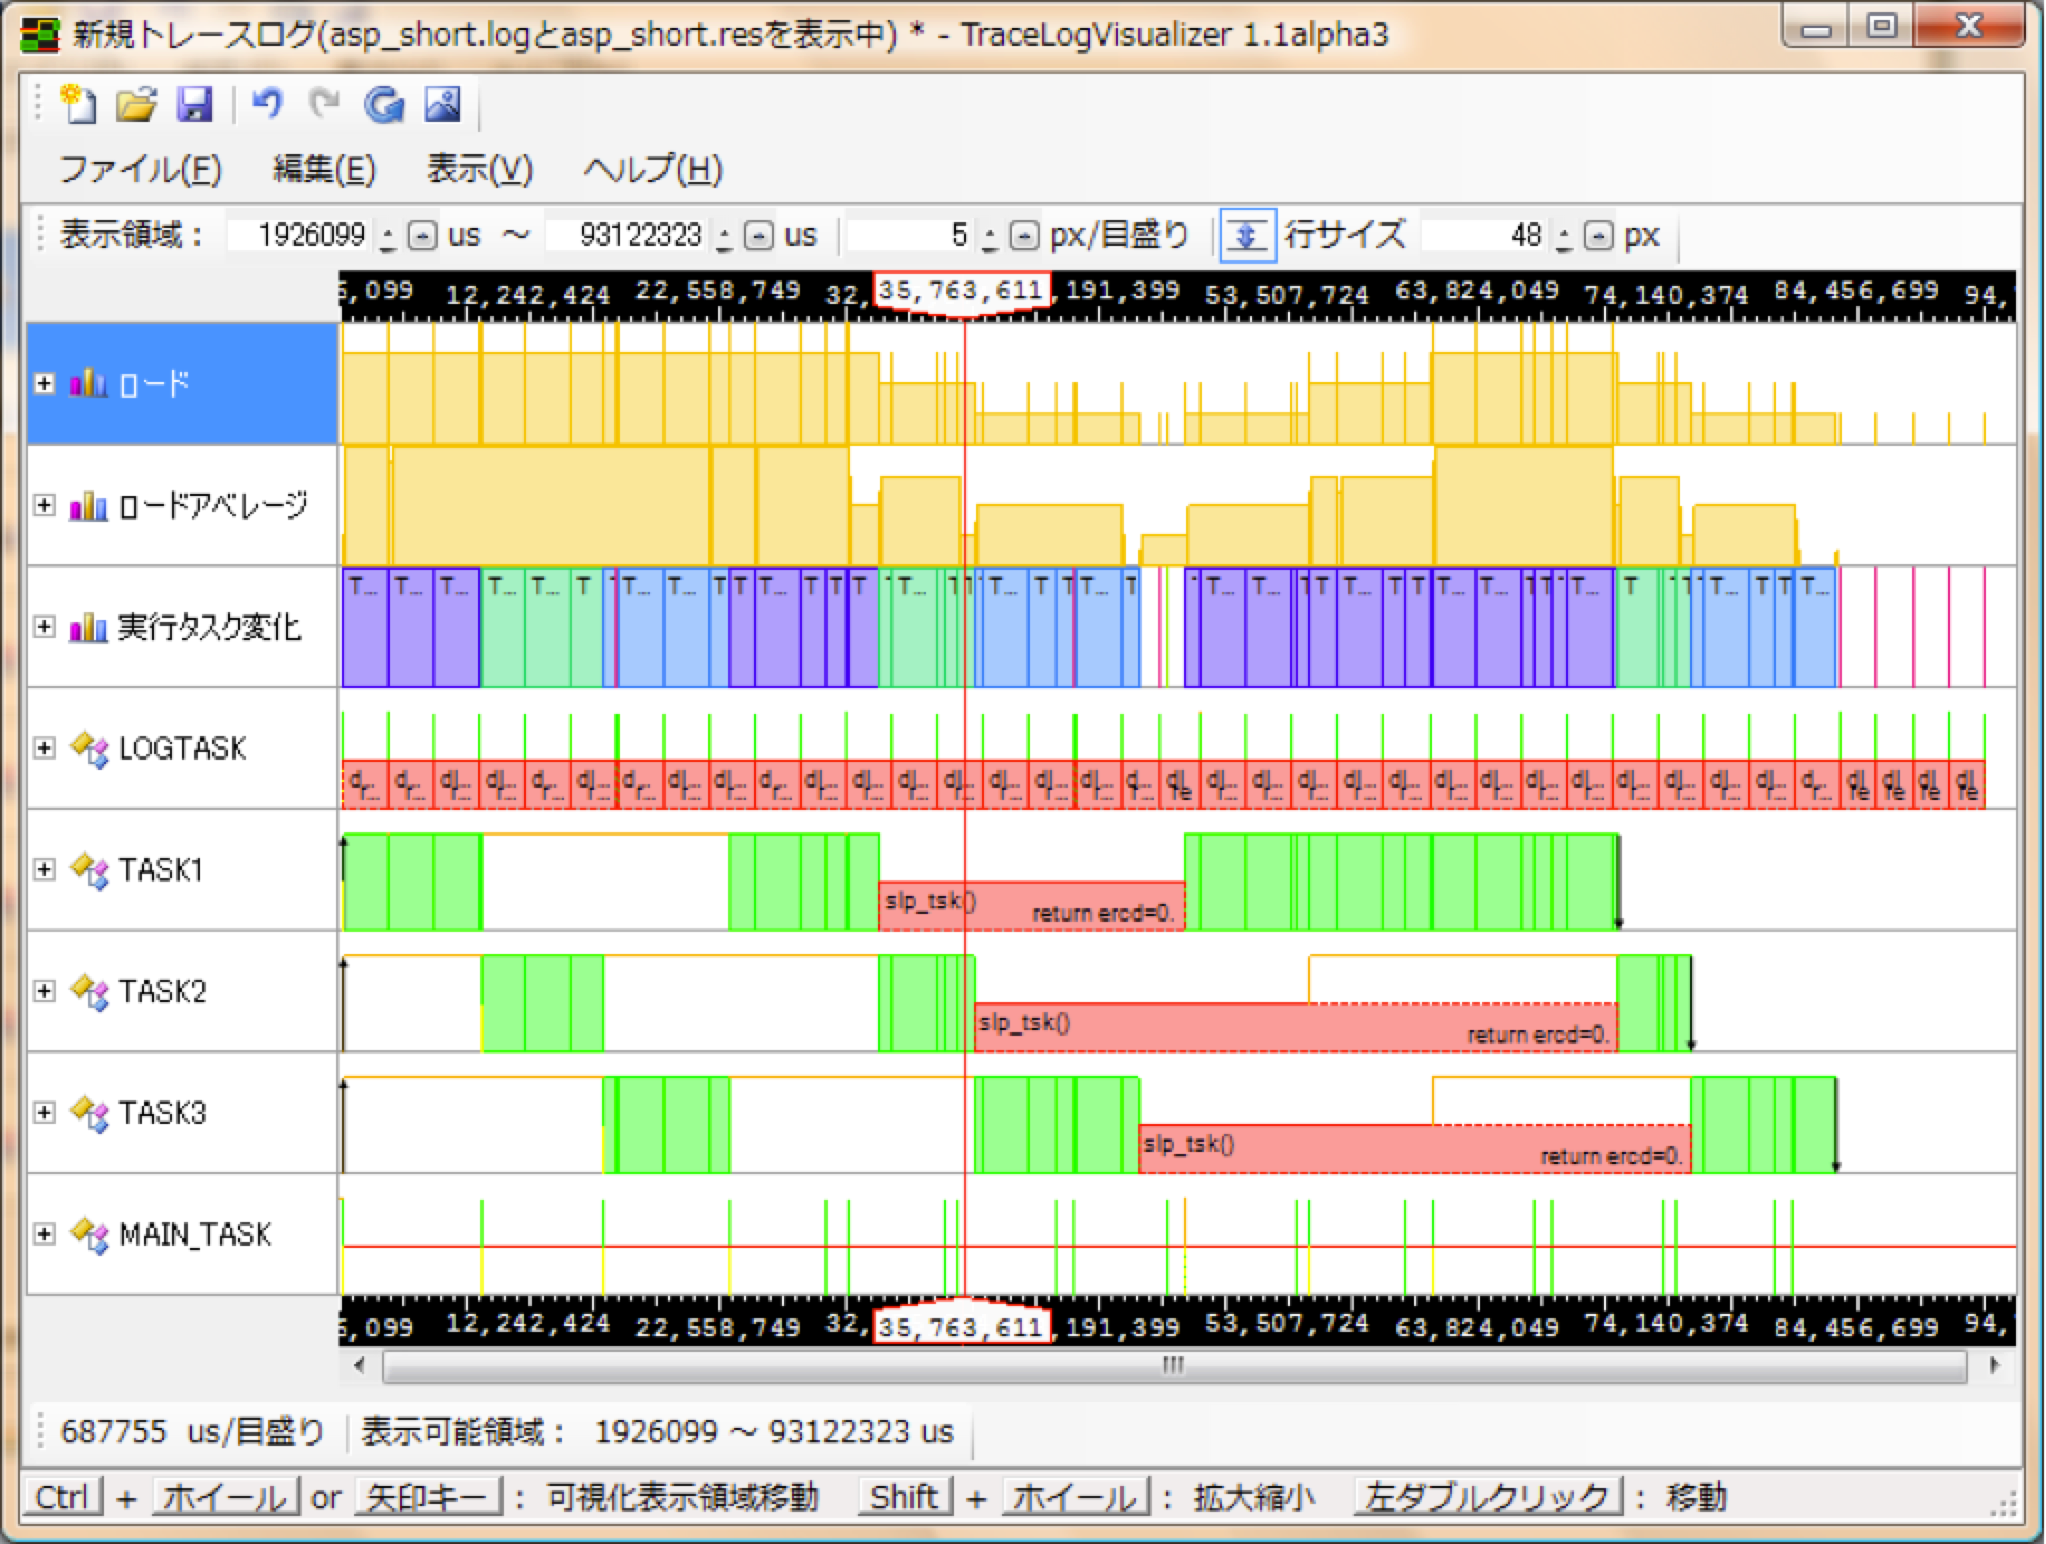
\includegraphics[width=10cm]{cpu.png}
\caption{CPUロード・ロードアベレージの可視化表示の例}\label{fig:cpu-use}
\end{figure}

